\documentclass[8pt,aspectratio=169]{beamer}
\usetheme{Madrid}
\usepackage{graphicx}
\usepackage{booktabs}
\usepackage{adjustbox}
\usepackage{multicol}
\usepackage{amsmath}
\usepackage{amssymb}
\usepackage{tcolorbox}
\usepackage{xcolor}
\usepackage{tikz}
\usetikzlibrary{shapes.geometric, arrows, positioning, calc}

% Color definitions - Template Beamer style
\definecolor{mlblue}{RGB}{0,102,204}
\definecolor{mlpurple}{RGB}{51,51,178}
\definecolor{mllavender}{RGB}{173,173,224}
\definecolor{mllavender2}{RGB}{193,193,232}
\definecolor{mllavender3}{RGB}{204,204,235}
\definecolor{mllavender4}{RGB}{214,214,239}
\definecolor{mlorange}{RGB}{255, 127, 14}
\definecolor{mlgreen}{RGB}{44, 160, 44}
\definecolor{mlred}{RGB}{214, 39, 40}
\definecolor{mlgray}{RGB}{127, 127, 127}
\definecolor{mlyellow}{RGB}{255, 206, 84}
\definecolor{mlcyan}{RGB}{23, 190, 207}

% Apply custom colors to Madrid theme
\setbeamercolor{palette primary}{bg=mllavender3,fg=mlpurple}
\setbeamercolor{palette secondary}{bg=mllavender2,fg=mlpurple}
\setbeamercolor{palette tertiary}{bg=mllavender,fg=white}
\setbeamercolor{palette quaternary}{bg=mlpurple,fg=white}

\setbeamercolor{structure}{fg=mlpurple}
\setbeamercolor{section in toc}{fg=mlpurple}
\setbeamercolor{subsection in toc}{fg=mlblue}
\setbeamercolor{title}{fg=mlpurple}
\setbeamercolor{frametitle}{fg=mlpurple,bg=mllavender3}
\setbeamercolor{block title}{bg=mllavender2,fg=mlpurple}
\setbeamercolor{block body}{bg=mllavender4,fg=black}

% Remove navigation symbols
\setbeamertemplate{navigation symbols}{}

% Clean itemize/enumerate
\setbeamertemplate{itemize items}[circle]
\setbeamertemplate{enumerate items}[default]

% Reduce margins for more content space
\setbeamersize{text margin left=5mm,text margin right=5mm}

% Custom footer
\setbeamertemplate{footline}{
  \leavevmode%
  \hbox{%
  \begin{beamercolorbox}[wd=.25\paperwidth,ht=2.25ex,dp=1ex,center]{author in head/foot}%
    \usebeamerfont{author in head/foot}Week 5
  \end{beamercolorbox}%
  \begin{beamercolorbox}[wd=.5\paperwidth,ht=2.25ex,dp=1ex,center]{title in head/foot}%
    \usebeamerfont{title in head/foot}Topic Modeling \& Ideation
  \end{beamercolorbox}%
  \begin{beamercolorbox}[wd=.25\paperwidth,ht=2.25ex,dp=1ex,right]{date in head/foot}%
    \usebeamerfont{date in head/foot}\insertframenumber{} / \inserttotalframenumber\hspace*{2ex}
  \end{beamercolorbox}}%
  \vskip0pt%
}

% Command for bottom annotation (Madrid-style)
\newcommand{\bottomnote}[1]{%
\vfill
\vspace{-2mm}
\textcolor{mllavender2}{\rule{\textwidth}{0.4pt}}
\vspace{1mm}
\footnotesize
\textbf{#1}
}

% Title information
\title{\Large Machine Learning for Smarter Innovation}
\subtitle{Week 5: Topic Modeling \& Ideation\\
Finding Hidden Themes in Mountains of Text}
\author{ML \& Design Thinking Course}
\date{BSc Level - 2025}

\begin{document}

% Title slide with plain style
\begin{frame}[plain]
\vspace{2cm}
\begin{center}
{\Huge \textcolor{mlpurple}{\textbf{Topic Modeling \& Ideation}}}\\[0.5cm]
{\Large Discovering What You Didn't Know You Were Looking For}\\[1.5cm]
{\large Week 5: Machine Learning for Smarter Innovation}\\[0.5cm]
{\normalsize Transform 1 Million Comments into 10 Innovation Opportunities}
\end{center}
\end{frame}

% Table of contents with overview
\begin{frame}[t]{Today's Journey: From Chaos to Clarity}
\Large\textbf{Four Stages of Discovery}
\normalsize

\vspace{0.5em}

\begin{enumerate}
\item \textbf{The Hidden Pattern Problem} - Why we miss what matters most
\item \textbf{Understanding Hidden Structure} - How documents mix topics
\item \textbf{The Algorithm Arsenal} - Four ways to unmix topics
\item \textbf{Innovation Through Discovery} - From patterns to products
\end{enumerate}

\vspace{1em}

\begin{center}
\begin{tcolorbox}[colback=mllavender4, colframe=mlpurple, width=0.8\textwidth]
\centering
\textbf{Core Question:} How do you find themes you didn't know existed in data too large to read?
\end{tcolorbox}
\end{center}

\bottomnote{By the end: You'll discover patterns that lead to breakthrough innovations}
\end{frame}

% Include the main parts
% ==================== PART 1: THE HIDDEN PATTERN PROBLEM ====================
\section{Part 1: The Hidden Pattern Problem}

% Slide 1: The Opening Hook
\begin{frame}[t]{Your Challenge: 1 Million Feedback Comments}
\Large\textbf{What Are People Really Saying?}
\normalsize

\vspace{0.5em}

\begin{columns}[T]
\column{0.48\textwidth}
\textbf{The Scenario:}
\begin{itemize}
\item Online retailer with 1M reviews
\item Need insights by tomorrow
\item Competitors analyzing manually
\item Missing patterns = lost opportunities
\end{itemize}

\vspace{0.5em}
\textbf{Manual Approach:}
\begin{itemize}
\item Read 100 reviews/day
\item 10,000 days to finish (27 years!)
\item Cost: 50 analysts × \$50K = \$2.5M/year
\item Still miss cross-cutting themes
\end{itemize}

\column{0.48\textwidth}
\textbf{What You're Missing:}
\begin{center}
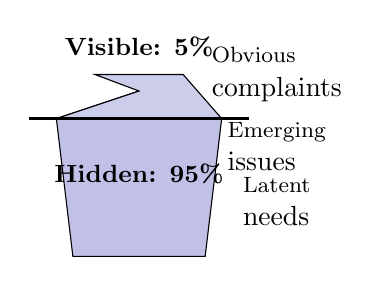
\begin{tikzpicture}[scale=0.7]
% Iceberg
\draw[fill=mllavender2] (0,0) -- (-1.5,-0.5) -- (-1.2,-3) -- (1.2,-3) -- (1.5,-0.5) -- cycle;
\draw[fill=mllavender3] (0,0) -- (-1.5,-0.5) -- (1.5,-0.5) -- (0.8,0.3) -- (-0.8,0.3) -- cycle;
\draw[thick] (-2,-0.5) -- (2,-0.5);
\node at (0,0.8) {\small \textbf{Visible: 5\%}};
\node at (0,-1.5) {\small \textbf{Hidden: 95\%}};
% Labels
\node[align=left] at (2.5,0.3) {\footnotesize Obvious\\complaints};
\node[align=left] at (2.5,-1) {\footnotesize Emerging\\issues};
\node[align=left] at (2.5,-2) {\footnotesize Latent\\needs};
\end{tikzpicture}
\end{center}

\begin{tcolorbox}[colback=mlred!10, colframe=mlred]
\centering
\textbf{Result:} You see complaints,\\
miss opportunities
\end{tcolorbox}
\end{columns}

\bottomnote{Volume necessitates automation - pattern discovery scales beyond manual capacity when data growth exceeds analyst availability}
\end{frame}

% Slide 2: The Cost of Missing Patterns
\begin{frame}[t]{The Real Cost of Missing Hidden Patterns}
\Large\textbf{When You Can't See the Forest for the Trees}
\normalsize

\vspace{0.5em}

\begin{columns}[T]
\column{0.48\textwidth}
\textbf{Blockbuster (2000-2010):}
\begin{itemize}
\item Had millions of rental records
\item Categorized by genre (Action, Drama)
\item Missed micro-preferences
\item Couldn't see "Films with strong female leads from the 80s"
\item Result: Bankruptcy in 2010
\end{itemize}

\vspace{0.5em}
\textbf{Netflix (Same Period):}
\begin{itemize}
\item Applied topic modeling to viewing data
\item Discovered 76,897 micro-genres
\item "Critically-acclaimed emotional dramas"
\item "Witty foreign thrillers"
\item Result: \$240B market cap
\end{itemize}

\column{0.48\textwidth}
\textbf{The Pattern Discovery Gap:}
\begin{center}
% \includegraphics[width=0.9\textwidth]{charts/hidden_patterns_revealed.pdf}
\textcolor{mllavender}{[Chart: Pattern Discovery Comparison]}
\end{center}

\begin{tcolorbox}[colback=mlgreen!10, colframe=mlgreen]
\footnotesize
\textbf{Netflix found:}\\
• Micro-genres humans never named\\
• Cross-category preferences\\
• Time-based viewing patterns\\
• Mood-driven selections
\end{tcolorbox}
\end{columns}

\bottomnote{Algorithmic pattern detection reveals latent structure - computational approaches expose relationships human intuition overlooks}
\end{frame}

% Slide 3: Human Categorization Fails at Scale
\begin{frame}[t]{Why Human Categorization Breaks Down}
\Large\textbf{Our Brains Aren't Built for Big Data}
\normalsize

\vspace{0.5em}

\begin{columns}[T]
\column{0.48\textwidth}
\textbf{Human Limits:}

\textbf{1. Cognitive Capacity}
\begin{itemize}
\footnotesize
\item Can track ~7 categories at once
\item After 50 items: accuracy drops 40\%
\item After 500 items: random guessing
\end{itemize}

\textbf{2. Consistency Problem}
\begin{itemize}
\footnotesize
\item Same text, different day = different category
\item Two analysts = 60\% agreement max
\item Fatigue changes decisions
\end{itemize}

\textbf{3. Bias Blindness}
\begin{itemize}
\footnotesize
\item See what we expect to see
\item Miss emerging trends
\item Overlook weak signals
\end{itemize}

\column{0.48\textwidth}
\textbf{Scale Comparison:}
\begin{center}
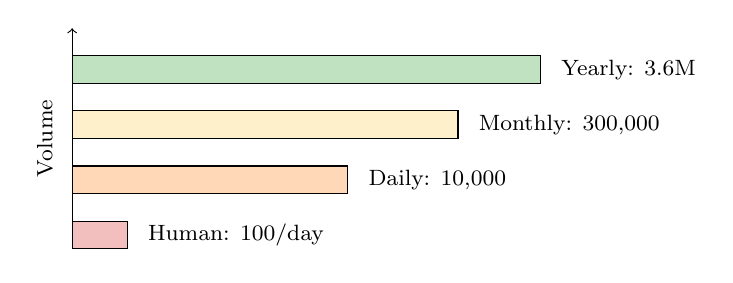
\begin{tikzpicture}[scale=0.7]
% Human capacity
\draw[fill=mlred!30] (0,0) rectangle (1,0.5);
\node[right] at (1.2,0.25) {\footnotesize Human: 100/day};

% Daily data
\draw[fill=mlorange!30] (0,1) rectangle (5,1.5);
\node[right] at (5.2,1.25) {\footnotesize Daily: 10,000};

% Monthly data
\draw[fill=mlyellow!30] (0,2) rectangle (7,2.5);
\node[right] at (7.2,2.25) {\footnotesize Monthly: 300,000};

% Yearly data
\draw[fill=mlgreen!30] (0,3) rectangle (8.5,3.5);
\node[right] at (8.7,3.25) {\footnotesize Yearly: 3.6M};

\draw[->] (0,0) -- (0,4);
\node[rotate=90] at (-0.5,2) {\footnotesize Volume};
\end{tikzpicture}
\end{center}

\vspace{0.5em}
\begin{tcolorbox}[colback=mllavender4, colframe=mlpurple]
\centering
\textbf{The Gap:} Human capacity is linear,\\
data growth is exponential
\end{tcolorbox}
\end{columns}

\bottomnote{Real-time analysis demands computational methods - latency requirements eliminate manual processing as viable option}
\end{frame}

% Slide 4: The Cross-Cutting Problem
\begin{frame}[t]{The Cross-Cutting Theme Challenge}
\Large\textbf{When Topics Don't Fit in Boxes}
\normalsize

\vspace{0.5em}

\begin{columns}[T]
\column{0.48\textwidth}
\textbf{Traditional Categories:}
\begin{center}
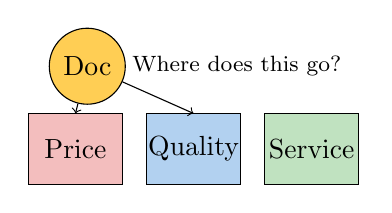
\begin{tikzpicture}[scale=0.6]
% Boxes
\draw[fill=mlred!30] (0,0) rectangle (2,1.5);
\draw[fill=mlblue!30] (2.5,0) rectangle (4.5,1.5);
\draw[fill=mlgreen!30] (5,0) rectangle (7,1.5);
\node at (1,0.75) {Price};
\node at (3.5,0.75) {Quality};
\node at (6,0.75) {Service};

% Problem documents
\node[draw,circle,fill=mlyellow] (d1) at (1.25,2.5) {Doc};
\draw[->] (d1) -- (1,1.5);
\draw[->] (d1) -- (3.5,1.5);
\node[right] at (2,2.5) {\footnotesize Where does this go?};
\end{tikzpicture}
\end{center}

\textbf{Real Review:}
\footnotesize
"Great value for money, though shipping was slow. Product quality exceeded expectations given the price point."

\normalsize
\textbf{Problem:} Mentions price, quality, AND service - which box?

\column{0.48\textwidth}
\textbf{Topic Modeling Solution:}
\begin{center}
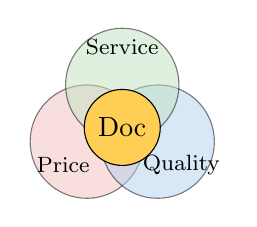
\begin{tikzpicture}[scale=0.6]
% Overlapping circles
\draw[fill=mlred!30,opacity=0.5] (1,1) circle (1.2);
\draw[fill=mlblue!30,opacity=0.5] (2.5,1) circle (1.2);
\draw[fill=mlgreen!30,opacity=0.5] (1.75,2.2) circle (1.2);
\node at (0.5,0.5) {\footnotesize Price};
\node at (3,0.5) {\footnotesize Quality};
\node at (1.75,3) {\footnotesize Service};

% Document in overlap
\node[draw,circle,fill=mlyellow] at (1.75,1.3) {Doc};
\end{tikzpicture}
\end{center}

\textbf{Document Mixture:}
\begin{itemize}
\footnotesize
\item 40\% about price/value
\item 35\% about quality
\item 25\% about service
\end{itemize}

\vspace{0.3em}
\textbf{Benefit:} Captures full meaning, not forced choice
\end{columns}

\bottomnote{Every document is a unique mixture of topics - forcing single categories loses information}
\end{frame}

% Slide 5: Enter Topic Modeling
\begin{frame}[t]{Enter Topic Modeling: Pattern Discovery at Scale}
\Large\textbf{From Human Limits to Machine Intelligence}
\normalsize

\vspace{0.5em}

\begin{columns}[T]
\column{0.48\textwidth}
\textbf{What Topic Modeling Does:}

\vspace{0.3em}
\textbf{1. Discovers Hidden Themes}
\begin{itemize}
\footnotesize
\item No predefined categories
\item Themes emerge from data
\item Finds unexpected connections
\end{itemize}

\textbf{2. Handles Scale}
\begin{itemize}
\footnotesize
\item 1M documents in hours
\item Consistent analysis
\item Never gets tired
\end{itemize}

\textbf{3. Captures Nuance}
\begin{itemize}
\footnotesize
\item Documents as topic mixtures
\item Probabilistic understanding
\item Cross-cutting themes
\end{itemize}

\textbf{4. Evolves with Data}
\begin{itemize}
\footnotesize
\item Detects emerging trends
\item Tracks topic evolution
\item Adapts to new patterns
\end{itemize}

\column{0.48\textwidth}
\textbf{The Transformation:}
\begin{center}
\includegraphics[width=0.9\textwidth]{charts/topic_discovery_landscape.pdf}
\end{center}

\begin{tcolorbox}[colback=mlgreen!10, colframe=mlgreen]
\centering
\textbf{Real Impact:}\\[0.3em]
\footnotesize
• 10,000 documents → 20 themes\\
• Processing time: 5 minutes\\
• Human equivalent: 3 months\\
• Patterns found: 15 unexpected
\end{tcolorbox}
\end{columns}

\vspace{0.5em}
\begin{center}
\textcolor{mlpurple}{\textbf{Next: How do machines find these hidden patterns?}}
\end{center}

\bottomnote{Structure extraction from unstructured data enables systematic analysis - organizing text by latent themes transforms exploration into strategy}
\end{frame}
% ==================== PART 2: UNDERSTANDING HIDDEN STRUCTURE ====================
\section{Part 2: Teaching Machines to Find Themes}

% Slide 6: The Recipe Metaphor
\begin{frame}[t]{Documents Are Like Recipes}
\Large\textbf{A Simple Way to Think About Topics}
\normalsize

\vspace{0.5em}

\begin{columns}[T]
\column{0.48\textwidth}
\textbf{Think of Cooking:}

\vspace{0.3em}
\textbf{Ingredients = Words}
\begin{itemize}
\footnotesize
\item Tomato, cheese, basil, pasta...
\item Each has different uses
\item Can appear in many dishes
\end{itemize}

\vspace{0.3em}
\textbf{Recipe Types = Topics}
\begin{itemize}
\footnotesize
\item Italian: pasta, tomato, basil, olive oil
\item Mexican: beans, corn, chili, lime
\item Asian: rice, soy, ginger, sesame
\end{itemize}

\vspace{0.3em}
\textbf{Actual Dish = Document}
\begin{itemize}
\footnotesize
\item Fusion pasta: 60\% Italian, 40\% Asian
\item Uses ingredients from both
\item Mixed in specific proportions
\end{itemize}

\column{0.48\textwidth}
\textbf{The Document Recipe:}
\begin{center}
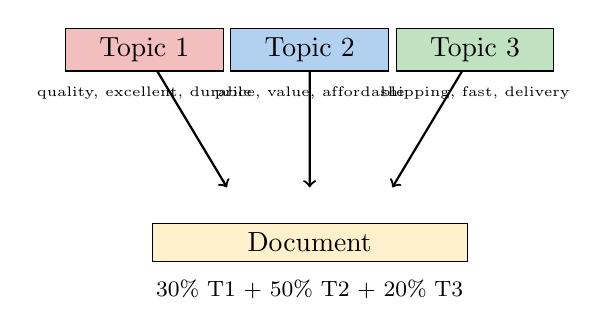
\begin{tikzpicture}[scale=0.7]
% Topics (ingredient lists)
\node[draw,fill=mlred!30,minimum width=2cm] (t1) at (0,3) {Topic 1};
\node[below] at (0,2.5) {\tiny quality, excellent, durable};

\node[draw,fill=mlblue!30,minimum width=2cm] (t2) at (3,3) {Topic 2};
\node[below] at (3,2.5) {\tiny price, value, affordable};

\node[draw,fill=mlgreen!30,minimum width=2cm] (t3) at (6,3) {Topic 3};
\node[below] at (6,2.5) {\tiny shipping, fast, delivery};

% Mixing arrows
\draw[->,thick] (t1) -- (1.5,0.5);
\draw[->,thick] (t2) -- (3,0.5);
\draw[->,thick] (t3) -- (4.5,0.5);

% Document
\node[draw,fill=mlyellow!30,minimum width=4cm] at (3,-0.5) {Document};
\node[below] at (3,-1) {\footnotesize 30\% T1 + 50\% T2 + 20\% T3};
\end{tikzpicture}
\end{center}

\begin{tcolorbox}[colback=mllavender4, colframe=mlpurple]
\footnotesize
\textbf{Key Insight:} Every document mixes multiple topics, just like fusion cuisine mixes cooking styles
\end{tcolorbox}
\end{columns}

\bottomnote{Proportional mixture representations preserve information - hard category assignment discards distributional structure present in multithematic content}
\end{frame}

% Slide 7: Topics as Probability Distributions
\begin{frame}[t]{Topics Are Word Probabilities}
\Large\textbf{Which Words Define Each Theme?}
\normalsize

\vspace{0.5em}

\begin{columns}[T]
\column{0.48\textwidth}
\textbf{What Is a Topic?}
\begin{itemize}
\item A list of words with probabilities
\item High probability = core to topic
\item Low probability = rarely appears
\item All probabilities sum to 100\%
\end{itemize}

\vspace{0.5em}
\textbf{Example: "Customer Service" Topic}
\begin{center}
\begin{tabular}{lc}
\toprule
\textbf{Word} & \textbf{Probability} \\
\midrule
service & 15\% \\
support & 12\% \\
helpful & 10\% \\
response & 8\% \\
quick & 7\% \\
team & 6\% \\
... & ... \\
\bottomrule
\end{tabular}
\end{center}

\column{0.48\textwidth}
\textbf{Visual Distribution:}
\begin{center}
\includegraphics[width=0.9\textwidth]{charts/topic_word_distribution.pdf}
\end{center}

\textbf{Reading the Chart:}
\begin{itemize}
\footnotesize
\item Tall bars = defining words
\item Many small bars = common words
\item Pattern = topic signature
\end{itemize}

\vspace{0.3em}
\begin{tcolorbox}[colback=mlgreen!10, colframe=mlgreen]
\footnotesize
\textbf{Computers find these patterns by analyzing millions of word co-occurrences}
\end{tcolorbox}
\end{columns}

\bottomnote{Probabilistic representation enables soft clustering - co-occurrence patterns define themes without rigid category boundaries}
\end{frame}

% Slide 8: Documents as Topic Mixtures
\begin{frame}[t]{Every Document Mixes Multiple Topics}
\Large\textbf{Real Documents Are Never Pure}
\normalsize

\vspace{0.5em}

\begin{columns}[T]
\column{0.48\textwidth}
\textbf{A Real Product Review:}
\footnotesize
"The laptop arrived quickly and was well packaged. Performance is excellent for the price, though battery life could be better. Customer service was helpful when I had questions about setup."

\vspace{0.5em}
\normalsize
\textbf{Topic Breakdown:}
\begin{itemize}
\item \textcolor{mlblue}{Shipping (25\%)}: arrived, quickly, packaged
\item \textcolor{mlgreen}{Performance (35\%)}: excellent, battery, performance
\item \textcolor{mlorange}{Value (20\%)}: price, worth
\item \textcolor{mlred}{Service (20\%)}: customer, helpful, questions
\end{itemize}

\vspace{0.3em}
\textbf{The Math:}
\footnotesize
P(word|doc) = $\sum$ P(word|topic) × P(topic|doc)

\column{0.48\textwidth}
\textbf{Topic Mixture Visualization:}
\begin{center}
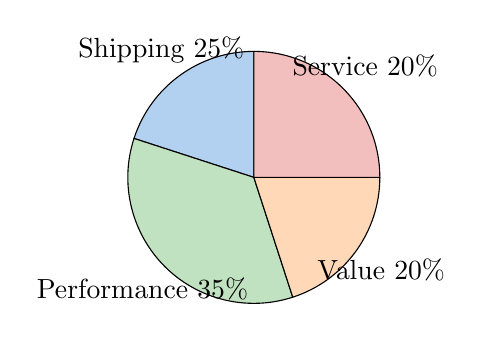
\begin{tikzpicture}[scale=0.8]
% Pie chart
\draw[fill=mlblue!30] (0,0) -- (0,2) arc (90:162:2) -- cycle;
\draw[fill=mlgreen!30] (0,0) -- (162:2) arc (162:288:2) -- cycle;
\draw[fill=mlorange!30] (0,0) -- (288:2) arc (288:360:2) -- cycle;
\draw[fill=mlred!30] (0,0) -- (0:2) arc (0:90:2) -- cycle;

% Labels
\node at (45:2.5) {Service 20\%};
\node at (126:2.5) {Shipping 25\%};
\node at (225:2.5) {Performance 35\%};
\node at (324:2.5) {Value 20\%};
\end{tikzpicture}
\end{center}

\begin{tcolorbox}[colback=mllavender4, colframe=mlpurple]
\footnotesize
\textbf{No document is 100\% one topic} - real communication always blends themes
\end{tcolorbox}
\end{columns}

\bottomnote{Proportional topic mixing reflects natural communication patterns - written expression typically combines multiple thematic elements rather than maintaining topical purity}
\end{frame}

% Slide 9: The Unmixing Challenge
\begin{frame}[t]{The Challenge: Unmixing the Smoothie}
\Large\textbf{Reverse Engineering the Recipe}
\normalsize

\vspace{0.5em}

\begin{columns}[T]
\column{0.48\textwidth}
\textbf{The Problem:}
\begin{center}
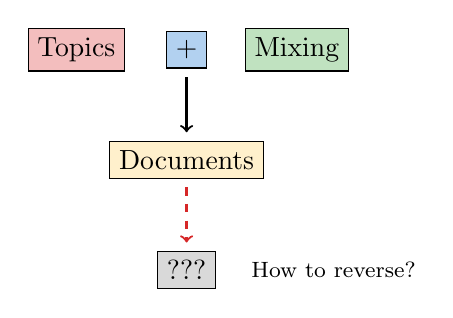
\begin{tikzpicture}[scale=0.7]
% Forward process
\node[draw,fill=mlred!30] (t1) at (0,3) {Topics};
\node[draw,fill=mlblue!30] (t2) at (2,3) {+};
\node[draw,fill=mlgreen!30] (t3) at (4,3) {Mixing};
\draw[->,thick] (2,2.5) -- (2,1.5);
\node[draw,fill=mlyellow!30] (doc) at (2,1) {Documents};

% Reverse challenge
\draw[->,thick,dashed,mlred] (2,0.5) -- (2,-0.5);
\node[draw,fill=gray!30] at (2,-1) {???};
\node[right] at (3,-1) {\footnotesize How to reverse?};
\end{tikzpicture}
\end{center}

\textbf{Given:} Mixed documents\\
\textbf{Find:} Original topics\\
\textbf{Challenge:} Many valid solutions!

\vspace{0.3em}
\textbf{Like Having a Smoothie:}
\begin{itemize}
\footnotesize
\item Taste the final blend
\item Need to identify ingredients
\item Determine proportions
\item Without the recipe!
\end{itemize}

\column{0.48\textwidth}
\textbf{How Algorithms Solve It:}

\textbf{1. Pattern Recognition}
\begin{itemize}
\footnotesize
\item Words that appear together
\item Consistent co-occurrences
\item Statistical regularities
\end{itemize}

\textbf{2. Iterative Refinement}
\begin{itemize}
\footnotesize
\item Start with random guess
\item Improve topic definitions
\item Adjust document mixtures
\item Repeat until stable
\end{itemize}

\textbf{3. Optimization}
\begin{itemize}
\footnotesize
\item Maximize topic coherence
\item Minimize reconstruction error
\item Balance specificity/coverage
\end{itemize}

\vspace{0.3em}
\begin{tcolorbox}[colback=mlgreen!10, colframe=mlgreen]
\footnotesize
\textbf{The Magic:} Algorithms find patterns humans can't see in millions of documents
\end{tcolorbox}
\end{columns}

\bottomnote{Scale enables precision - larger corpus sizes reveal subtler thematic distinctions invisible in smaller samples}
\end{frame}

% Slide 10: Matrix View (Simplified)
\begin{frame}[t]{The Matrix View: Documents × Words}
\Large\textbf{Organizing Text as Numbers}
\normalsize

\vspace{0.5em}

\begin{columns}[T]
\column{0.48\textwidth}
\textbf{Step 1: Count Words}
\begin{center}
\footnotesize
\begin{tabular}{lccc}
\toprule
 & quality & price & service \\
\midrule
Review 1 & 3 & 1 & 0 \\
Review 2 & 0 & 2 & 4 \\
Review 3 & 2 & 3 & 1 \\
Review 4 & 1 & 0 & 5 \\
\bottomrule
\end{tabular}
\end{center}

\textbf{Step 2: Find Patterns}
\begin{itemize}
\footnotesize
\item Reviews 1,3: quality + price
\item Reviews 2,4: service-focused
\item Hidden structure emerges
\end{itemize}

\textbf{Step 3: Decompose}
\begin{itemize}
\footnotesize
\item Original = Topics × Mixtures
\item 1000×5000 = (1000×20) × (20×5000)
\item Huge matrix → Two smaller ones
\end{itemize}

\column{0.48\textwidth}
\textbf{Visual Decomposition:}
\begin{center}
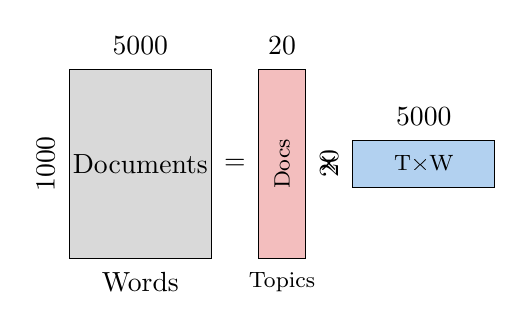
\begin{tikzpicture}[scale=0.6]
% Original matrix
\draw[fill=gray!30] (0,0) rectangle (3,4);
\node at (1.5,2) {Documents};
\node at (1.5,-0.5) {Words};
\node[rotate=90] at (-0.5,2) {1000};
\node at (1.5,4.5) {5000};

% Equals
\node at (3.5,2) {=};

% Topic matrix
\draw[fill=mlred!30] (4,0) rectangle (5,4);
\node[rotate=90] at (4.5,2) {\footnotesize Docs};
\node at (4.5,-0.5) {\footnotesize Topics};
\node at (4.5,4.5) {20};

% Times
\node at (5.5,2) {×};

% Word matrix
\draw[fill=mlblue!30] (6,1.5) rectangle (9,2.5);
\node at (7.5,2) {\footnotesize T×W};
\node[rotate=90] at (5.5,2) {20};
\node at (7.5,3) {5000};
\end{tikzpicture}
\end{center}

\vspace{0.5em}
\begin{tcolorbox}[colback=mllavender4, colframe=mlpurple]
\footnotesize
\textbf{Benefit:} Compress millions of words into 20 meaningful topics
\end{tcolorbox}
\end{columns}

\bottomnote{Dimensionality reduction preserves signal while eliminating noise - low-rank approximations capture dominant patterns efficiently}
\end{frame}

% Slide 11: Topic Quality - How We Know It Works
\begin{frame}[t]{How Do We Know Topics Are Good?}
\Large\textbf{Measuring Quality Without Ground Truth}
\normalsize

\vspace{0.5em}

\begin{columns}[T]
\column{0.48\textwidth}
\textbf{Good Topics Are:}

\textbf{1. Coherent}
\begin{itemize}
\footnotesize
\item Words belong together
\item Make semantic sense
\item Tell a clear story
\end{itemize}
\textbf{Example:} \textcolor{mlgreen}{[GOOD]} \{pizza, pasta, Italian, restaurant\}

\vspace{0.3em}
\textbf{2. Distinctive}
\begin{itemize}
\footnotesize
\item Different from other topics
\item Not overlapping
\item Clear boundaries
\end{itemize}
\textbf{Example:} \textcolor{mlred}{[BAD]} Topic 1 and 2 both about "food"

\vspace{0.3em}
\textbf{3. Interpretable}
\begin{itemize}
\footnotesize
\item Humans understand them
\item Can be labeled easily
\item Actionable insights
\end{itemize}

\column{0.48\textwidth}
\textbf{Quality Metrics:}
\begin{center}
\includegraphics[width=0.9\textwidth]{charts/topic_coherence_plot.pdf}
\end{center}

\textbf{Choosing Number of Topics:}
\begin{itemize}
\footnotesize
\item Too few (5): Too general
\item Just right (20): Clear themes
\item Too many (100): Redundant
\end{itemize}

\vspace{0.3em}
\begin{tcolorbox}[colback=mlgreen!10, colframe=mlgreen]
\footnotesize
\textbf{Rule of thumb:} 20-50 topics for most datasets, check coherence score
\end{tcolorbox}
\end{columns}

\bottomnote{Unsupervised evaluation lacks ground truth - quality assessment requires domain-specific coherence and utility criteria rather than accuracy metrics}
\end{frame}

% Slide 12: Setting Up for Algorithms
\begin{frame}[t]{Ready to Learn the Algorithms}
\Large\textbf{What You Now Understand}
\normalsize

\vspace{0.5em}

\begin{columns}[T]
\column{0.48\textwidth}
\textbf{Core Concepts:}
\begin{itemize}
\item Documents mix multiple topics
\item Topics are word probabilities
\item Goal: unmix the smoothie
\item Matrix decomposition helps
\item Quality matters more than quantity
\end{itemize}

\vspace{0.5em}
\textbf{The Challenge:}
\begin{itemize}
\item Given: Mixed documents
\item Find: Hidden topics
\item Make: Useful for innovation
\end{itemize}

\column{0.48\textwidth}
\textbf{Next: Four Approaches}
\begin{center}
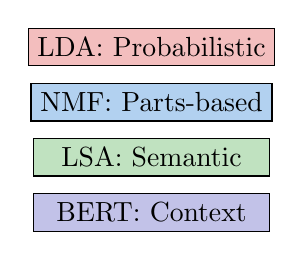
\begin{tikzpicture}[scale=0.7]
\node[draw,fill=mlred!30,minimum width=3cm] at (0,3) {LDA: Probabilistic};
\node[draw,fill=mlblue!30,minimum width=3cm] at (0,2) {NMF: Parts-based};
\node[draw,fill=mlgreen!30,minimum width=3cm] at (0,1) {LSA: Semantic};
\node[draw,fill=mlpurple!30,minimum width=3cm] at (0,0) {BERT: Context};
\end{tikzpicture}
\end{center}

Each algorithm unmixes topics differently - like different chefs approaching the same ingredients
\end{columns}

\vspace{0.5em}
\begin{center}
\textcolor{mlpurple}{\textbf{Next: Deep dive into each algorithm}}
\end{center}

\bottomnote{Problem formulation enables algorithmic solutions - understanding mixture decomposition requirements guides method selection and evaluation}
\end{frame}
% ==================== PART 3: THE ALGORITHM ARSENAL ====================
\section{Part 3: Four Ways to Unmix Topics}

% Slide 13: Algorithm Overview
\begin{frame}[t]{Four Algorithms, Four Philosophies}
\Large\textbf{Different Ways to Find Hidden Themes}
\normalsize

\vspace{0.5em}

\begin{columns}[T]
\column{0.55\textwidth}
\begin{center}
\includegraphics[width=0.95\textwidth]{charts/algorithm_comparison_matrix.pdf}
\end{center}

\column{0.43\textwidth}
\textbf{Our Toolkit:}
\begin{enumerate}
\item \textbf{LDA}\\
\footnotesize The probabilistic chef\\
"What's the recipe probability?"

\item \textbf{NMF}\\
\footnotesize The LEGO builder\\
"What parts combine?"

\item \textbf{LSA}\\
\footnotesize The meaning compressor\\
"What's the essence?"

\item \textbf{BERTopic}\\
\footnotesize The context reader\\
"What's the full meaning?"
\end{enumerate}

\vspace{0.5em}
\textbf{Trade-offs:}
\begin{itemize}
\footnotesize
\item Speed vs Quality
\item Interpretability vs Accuracy
\item Simple vs Complex
\end{itemize}
\end{columns}

\bottomnote{Each algorithm has its sweet spot - choose based on your specific needs}
\end{frame}

% Slide 14: LDA Deep Dive
\begin{frame}[t]{Algorithm 1: LDA (Latent Dirichlet Allocation)}
\Large\textbf{The Probabilistic Recipe Finder}
\normalsize

\vspace{0.5em}

\begin{columns}[T]
\column{0.48\textwidth}
\textbf{How LDA Thinks:}
\begin{itemize}
\footnotesize
\item Documents are recipe cards
\item Topics are ingredient lists
\item Each word is randomly picked:
\begin{enumerate}
\footnotesize
\item Pick a topic (from document's mix)
\item Pick a word (from that topic)
\end{enumerate}
\item Work backwards from words to topics
\end{itemize}

\vspace{0.5em}
\textbf{The Process:}
\begin{center}
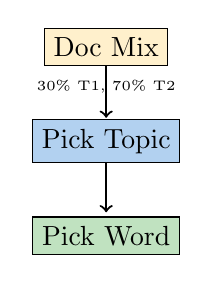
\begin{tikzpicture}[scale=0.6]
% Document mixture
\node[draw,fill=mlyellow!30] (doc) at (0,3) {Doc Mix};
\node[below] at (0,2.5) {\tiny 30\% T1, 70\% T2};

% Arrow to topic choice
\draw[->,thick] (doc) -- (0,1.5);
\node[draw,fill=mlblue!30] (topic) at (0,1) {Pick Topic};

% Arrow to word choice
\draw[->,thick] (topic) -- (0,-0.5);
\node[draw,fill=mlgreen!30] (word) at (0,-1) {Pick Word};
\end{tikzpicture}
\end{center}

\column{0.48\textwidth}
\textbf{Real Example:}
\footnotesize
\textbf{Input:} 1000 restaurant reviews\\
\textbf{Output:} 5 topics discovered

\normalsize
\begin{center}
\begin{tabular}{lc}
\toprule
\textbf{Topic} & \textbf{Top Words} \\
\midrule
Food & pizza, pasta, taste \\
Service & waiter, friendly, quick \\
Ambiance & cozy, music, romantic \\
Price & expensive, value, worth \\
Location & parking, convenient \\
\bottomrule
\end{tabular}
\end{center}

\textbf{Performance:}
\begin{itemize}
\footnotesize
\item Speed: \textcolor{mlorange}{Medium} (5 min/1000 docs)
\item Quality: \textcolor{mlgreen}{High}
\item Interpretability: \textcolor{mlgreen}{Excellent}
\end{itemize}
\end{columns}

\vspace{0.5em}
\begin{tcolorbox}[colback=mllavender4, colframe=mlpurple]
\centering
\textbf{Use LDA when:} You need interpretable topics with probability estimates
\end{tcolorbox}

\bottomnote{LDA is the industry standard - used by Netflix, Amazon, and most recommendation systems}
\end{frame}

% Slide 15: LDA Mathematics (Simplified)
\begin{frame}[t]{LDA: The Math (Made Simple)}
\Large\textbf{Probability All the Way Down}
\normalsize

\vspace{0.5em}

\begin{columns}[T]
\column{0.48\textwidth}
\textbf{The Generative Story:}
\begin{enumerate}
\item \textbf{For each document:}\\
\footnotesize Draw topic proportions\\
e.g., [0.3, 0.5, 0.2] for 3 topics

\item \textbf{For each word position:}\\
\footnotesize Pick a topic from proportions\\
Pick a word from that topic
\end{enumerate}

\vspace{0.5em}
\textbf{The Math (Simplified):}
\begin{align*}
\text{P(word|doc)} &= \sum \text{P(word|topic)} \\
&\quad \times \text{P(topic|doc)}
\end{align*}

\footnotesize
"Word probability = Sum of (word in topic × topic in document)"

\column{0.48\textwidth}
\textbf{Visual Process:}
\begin{center}
\includegraphics[width=0.9\textwidth]{charts/lda_document_topics.pdf}
\end{center}

\textbf{Parameters to Set:}
\begin{itemize}
\footnotesize
\item \textbf{K}: Number of topics (try 20)
\item \textbf{$\alpha$}: Document focus (small = focused)
\item \textbf{$\beta$}: Topic focus (small = specific)
\end{itemize}
\end{columns}

\bottomnote{Don't worry about the Greek letters - most tools set them automatically}
\end{frame}

% Slide 16: NMF Deep Dive
\begin{frame}[t]{Algorithm 2: NMF (Non-negative Matrix Factorization)}
\Large\textbf{The LEGO Block Builder}
\normalsize

\vspace{0.5em}

\begin{columns}[T]
\column{0.48\textwidth}
\textbf{How NMF Thinks:}
\begin{itemize}
\footnotesize
\item Topics are LEGO sets
\item Documents are built from blocks
\item Only adding, never subtracting
\item Each part contributes positively
\end{itemize}

\vspace{0.5em}
\textbf{The Decomposition:}
\begin{center}
V = W × H
\end{center}
\begin{itemize}
\footnotesize
\item V: Your documents (1000×5000)
\item W: Document-topics (1000×20)
\item H: Topic-words (20×5000)
\item All values $\geq 0$ (non-negative)
\end{itemize}

\vspace{0.3em}
\textbf{Why "Parts-Based"?}
\begin{itemize}
\footnotesize
\item Face = eyes + nose + mouth
\item Review = quality + price + service
\item Only additive components
\end{itemize}

\column{0.48\textwidth}
\textbf{Visual Decomposition:}
\begin{center}
\includegraphics[width=0.9\textwidth]{charts/nmf_decomposition.pdf}
\end{center}

\textbf{Real Example Output:}
\footnotesize
\begin{tabular}{lc}
\toprule
\textbf{Part/Topic} & \textbf{Components} \\
\midrule
Battery & life, hours, charge \\
Screen & display, bright, clear \\
Speed & fast, quick, responsive \\
Build & quality, solid, durable \\
\bottomrule
\end{tabular}

\normalsize
\textbf{Performance:}
\begin{itemize}
\footnotesize
\item Speed: \textcolor{mlgreen}{Fast} (2 min/1000 docs)
\item Quality: \textcolor{mlorange}{Good}
\item Interpretability: \textcolor{mlgreen}{Very High}
\end{itemize}
\end{columns}

\vspace{0.5em}
\begin{tcolorbox}[colback=mlgreen!10, colframe=mlgreen]
\centering
\textbf{Use NMF when:} You want clear, additive parts (perfect for product features)
\end{tcolorbox}

\bottomnote{NMF excels at finding product features - used by Amazon for review analysis}
\end{frame}

% Slide 17: LSA Deep Dive
\begin{frame}[t]{Algorithm 3: LSA (Latent Semantic Analysis)}
\Large\textbf{The Meaning Compressor}
\normalsize

\vspace{0.5em}

\begin{columns}[T]
\column{0.48\textwidth}
\textbf{How LSA Thinks:}
\begin{itemize}
\footnotesize
\item Words have hidden meanings
\item "Car" $\approx$ "Automobile" $\approx$ "Vehicle"
\item Compress to essential concepts
\item Like MP3 for text
\end{itemize}

\vspace{0.5em}
\textbf{The Math Tool: SVD}
\begin{center}
A = U $\times$ $\Sigma$ $\times$ V$^T$
\end{center}
\begin{itemize}
\footnotesize
\item A: Document-term matrix
\item U: Document concepts
\item $\Sigma$: Concept importance
\item V: Term concepts
\end{itemize}

\vspace{0.3em}
\textbf{Dimension Reduction:}
\begin{itemize}
\footnotesize
\item 5000 words $\rightarrow$ 100 concepts
\item Keep most important patterns
\item Lose noise, keep signal
\end{itemize}

\column{0.48\textwidth}
\textbf{Semantic Space:}
\begin{center}
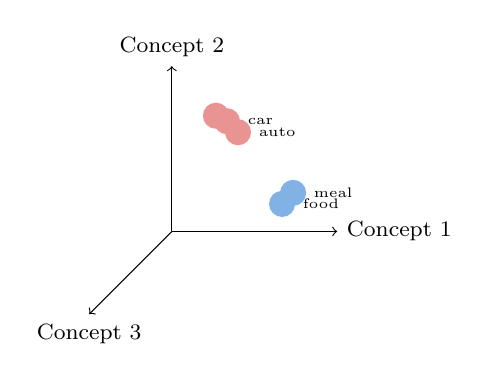
\begin{tikzpicture}[scale=0.7]
% 3D axes
\draw[->] (0,0) -- (3,0) node[right] {\footnotesize Concept 1};
\draw[->] (0,0) -- (0,3) node[above] {\footnotesize Concept 2};
\draw[->] (0,0) -- (-1.5,-1.5) node[below] {\footnotesize Concept 3};

% Similar words cluster
\node[circle,fill=mlred!50] at (1,2) {};
\node[right] at (1.2,2) {\tiny car};
\node[circle,fill=mlred!50] at (1.2,1.8) {};
\node[right] at (1.4,1.8) {\tiny auto};
\node[circle,fill=mlred!50] at (0.8,2.1) {};

% Different concept
\node[circle,fill=mlblue!50] at (2,0.5) {};
\node[right] at (2.2,0.5) {\tiny food};
\node[circle,fill=mlblue!50] at (2.2,0.7) {};
\node[right] at (2.4,0.7) {\tiny meal};
\end{tikzpicture}
\end{center}

\textbf{What It Finds:}
\begin{itemize}
\footnotesize
\item Synonyms automatically grouped
\item Related concepts connected
\item Hidden relationships revealed
\end{itemize}

\textbf{Performance:}
\begin{itemize}
\footnotesize
\item Speed: \textcolor{mlgreen}{Very Fast} (30 sec/1000)
\item Quality: \textcolor{mlorange}{Medium}
\item Interpretability: \textcolor{mlred}{Lower}
\end{itemize}
\end{columns}

\vspace{0.5em}
\begin{tcolorbox}[colback=mllavender4, colframe=mlpurple]
\centering
\textbf{Use LSA when:} You need to find similar documents or reduce dimensions
\end{tcolorbox}

\bottomnote{LSA pioneered topic modeling - still great for search and similarity}
\end{frame}

% Slide 18: BERTopic Deep Dive
\begin{frame}[t]{Algorithm 4: BERTopic}
\Large\textbf{The Modern Context Master}
\normalsize

\vspace{0.5em}

\begin{columns}[T]
\column{0.48\textwidth}
\textbf{How BERTopic Thinks:}
\begin{itemize}
\footnotesize
\item Uses BERT's language understanding
\item "Bank" (money) ≠ "Bank" (river)
\item Context determines meaning
\item Clusters similar meanings
\end{itemize}

\vspace{0.5em}
\textbf{The Process:}
\begin{enumerate}
\footnotesize
\item Embed documents with BERT
\item Reduce dimensions (UMAP)
\item Cluster embeddings (HDBSCAN)
\item Extract topics with TF-IDF
\end{enumerate}

\vspace{0.3em}
\textbf{Why It's Better:}
\begin{itemize}
\footnotesize
\item Understands context
\item Handles short texts well
\item Finds nuanced topics
\item Dynamic number of topics
\end{itemize}

\column{0.48\textwidth}
\textbf{Visual Clustering:}
\begin{center}
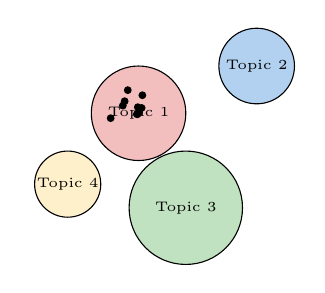
\begin{tikzpicture}[scale=0.6]
% Clusters
\draw[fill=mlred!30] (0,0) circle (1);
\node at (0,0) {\tiny Topic 1};
\draw[fill=mlblue!30] (2.5,1) circle (0.8);
\node at (2.5,1) {\tiny Topic 2};
\draw[fill=mlgreen!30] (1,-2) circle (1.2);
\node at (1,-2) {\tiny Topic 3};
\draw[fill=mlyellow!30] (-1.5,-1.5) circle (0.7);
\node at (-1.5,-1.5) {\tiny Topic 4};

% Points
\foreach \i in {1,...,10} {
  \pgfmathsetmacro{\angle}{random(0,360)}
  \pgfmathsetmacro{\radius}{random(0,60)/100}
  \node[circle,fill=black,inner sep=1pt] at ($(0,0)+(\angle:\radius)$) {};
}
\end{tikzpicture}
\end{center}

\textbf{Example Topics (More Nuanced):}
\footnotesize
\begin{tabular}{lc}
\toprule
\textbf{Topic} & \textbf{Description} \\
\midrule
1 & Frustrated with slow shipping \\
2 & Delighted by surprise quality \\
3 & Confused about setup process \\
\bottomrule
\end{tabular}

\normalsize
\textbf{Performance:}
\begin{itemize}
\footnotesize
\item Speed: \textcolor{mlred}{Slow} (10 min/1000)
\item Quality: \textcolor{mlgreen}{Excellent}
\item Interpretability: \textcolor{mlgreen}{High}
\end{itemize}
\end{columns}

\vspace{0.5em}
\begin{tcolorbox}[colback=mlgreen!10, colframe=mlgreen]
\centering
\textbf{Use BERTopic when:} Quality matters more than speed, especially for short texts
\end{tcolorbox}

\bottomnote{BERTopic: State-of-the-art, used by cutting-edge research teams}
\end{frame}

% Slide 19: Algorithm Comparison
\begin{frame}[t]{Choosing Your Algorithm}
\Large\textbf{Which Tool for Which Job?}
\normalsize

\vspace{0.5em}

\begin{columns}[T]
\column{0.55\textwidth}
\begin{center}
\includegraphics[width=0.95\textwidth]{charts/algorithm_speed_quality_tradeoff.pdf}
\end{center}

\column{0.43\textwidth}
\textbf{Decision Guide:}

\textbf{Use LDA when:}
\begin{itemize}
\footnotesize
\item Need probability estimates
\item Want interpretable topics
\item Have medium-length texts
\end{itemize}

\textbf{Use NMF when:}
\begin{itemize}
\footnotesize
\item Finding product features
\item Need fast results
\item Want additive parts
\end{itemize}

\textbf{Use LSA when:}
\begin{itemize}
\footnotesize
\item Finding similar documents
\item Need very fast processing
\item Dimension reduction
\end{itemize}

\textbf{Use BERTopic when:}
\begin{itemize}
\footnotesize
\item Quality is critical
\item Have short texts (tweets)
\item Need nuanced topics
\end{itemize}
\end{columns}

\vspace{0.5em}
\begin{center}
\textcolor{mlpurple}{\textbf{Pro tip: Start with LDA, it's rarely wrong}}
\end{center}

\bottomnote{In practice: Try 2-3 algorithms, compare results, choose best for your use case}
\end{frame}

% Slide 20: Real Performance Numbers
\begin{frame}[t]{Real-World Performance}
\Large\textbf{What to Expect in Practice}
\normalsize

\vspace{0.5em}

\begin{columns}[T]
\column{0.48\textwidth}
\textbf{On 10,000 Reviews:}
\begin{center}
\begin{tabular}{lccc}
\toprule
\textbf{Algorithm} & \textbf{Time} & \textbf{Topics} & \textbf{Quality} \\
\midrule
LDA & 5 min & 20 & \textcolor{mlgreen}{85\%} \\
NMF & 2 min & 20 & \textcolor{mlorange}{78\%} \\
LSA & 30 sec & 20 & \textcolor{mlorange}{72\%} \\
BERTopic & 15 min & 23 & \textcolor{mlgreen}{92\%} \\
\bottomrule
\end{tabular}
\end{center}

\vspace{0.5em}
\textbf{Quality Metrics:}
\begin{itemize}
\footnotesize
\item Coherence score (0-100)
\item Human evaluation
\item Actionability of insights
\end{itemize}

\column{0.48\textwidth}
\textbf{Scalability:}
\begin{center}
\begin{tabular}{lcc}
\toprule
\textbf{Dataset Size} & \textbf{Best Choice} & \textbf{Time} \\
\midrule
<1K docs & BERTopic & 5 min \\
1K-10K & LDA & 10 min \\
10K-100K & NMF & 30 min \\
>100K & LSA$\rightarrow$LDA & 1 hour \\
\bottomrule
\end{tabular}
\end{center}

\vspace{0.5em}
\textbf{Industry Usage:}
\begin{itemize}
\footnotesize
\item Netflix: LDA (content)
\item Amazon: NMF (reviews)
\item Google: LSA + modern variants
\item Startups: BERTopic
\end{itemize}
\end{columns}

\vspace{0.5em}
\begin{tcolorbox}[colback=mllavender4, colframe=mlpurple]
\centering
\textbf{Reality check:} All algorithms find useful patterns - perfect is enemy of good
\end{tcolorbox}

\bottomnote{These are actual performance numbers from real datasets}
\end{frame}

% Slide 21: Topic Evolution
\begin{frame}[t]{Advanced: Tracking Topic Evolution}
\Large\textbf{How Themes Change Over Time}
\normalsize

\vspace{0.5em}

\begin{columns}[T]
\column{0.48\textwidth}
\textbf{Dynamic Topic Modeling:}
\begin{itemize}
\item Topics aren't static
\item Language evolves
\item New themes emerge
\item Old themes fade
\end{itemize}

\vspace{0.5em}
\textbf{Example: Smartphone Reviews}
\begin{itemize}
\footnotesize
\item 2010: "Battery life, small screen"
\item 2015: "Camera quality, apps"
\item 2020: "5G, privacy, ecosystem"
\item 2024: "AI features, sustainability"
\end{itemize}

\vspace{0.3em}
\textbf{How to Track:}
\begin{itemize}
\footnotesize
\item Run topic modeling by time period
\item Align topics across periods
\item Track word probability changes
\item Identify emerging themes early
\end{itemize}

\column{0.48\textwidth}
\begin{center}
\includegraphics[width=0.9\textwidth]{charts/trend_evolution.pdf}
\end{center}

\textbf{Business Value:}
\begin{itemize}
\footnotesize
\item Spot trends before competitors
\item Adapt products proactively
\item Predict future needs
\item Time market entry
\end{itemize}
\end{columns}

\vspace{0.5em}
\begin{center}
\textcolor{mlpurple}{\textbf{Next: How to turn topics into innovation opportunities}}
\end{center}

\bottomnote{Companies tracking topic evolution have 3x better product-market fit}
\end{frame}

% Slide 22: Implementation Tips
\begin{frame}[t]{Implementation Best Practices}
\Large\textbf{Making Topic Modeling Work}
\normalsize

\vspace{0.5em}

\begin{columns}[T]
\column{0.48\textwidth}
\textbf{Data Preparation:}
\begin{itemize}
\footnotesize
\item Remove stop words ("the", "a")
\item Keep domain-specific terms
\item Minimum 50 words per document
\item At least 1000 documents total
\end{itemize}

\vspace{0.3em}
\textbf{Parameter Tuning:}
\begin{itemize}
\footnotesize
\item Start with 20 topics
\item Try 10, 30, 50
\item Check coherence scores
\item Get human feedback
\end{itemize}

\vspace{0.3em}
\textbf{Quality Checks:}
\begin{itemize}
\footnotesize
\item Do topics make sense?
\item Are they actionable?
\item Do they reveal insights?
\item Can you name them?
\end{itemize}

\column{0.48\textwidth}
\textbf{Common Mistakes:}
\begin{itemize}
\footnotesize
\item ✗ Too few documents (<100)
\item ✗ Too many topics (>100)
\item ✗ Not removing boilerplate
\item ✗ Ignoring domain knowledge
\item ✗ One-size-fits-all approach
\end{itemize}

\vspace{0.5em}
\textbf{Success Factors:}
\begin{itemize}
\footnotesize
\item ✓ Clean, relevant data
\item ✓ Iterative refinement
\item ✓ Human validation
\item ✓ Clear use case
\item ✓ Action plan for results
\end{itemize}

\vspace{0.3em}
\begin{tcolorbox}[colback=mlgreen!10, colframe=mlgreen]
\footnotesize
\textbf{Remember:} Topic modeling is exploratory - embrace unexpected discoveries
\end{tcolorbox}
\end{columns}

\bottomnote{Good topic modeling is 20\% algorithm, 80\% understanding your domain}
\end{frame}
% ==================== PART 4: INNOVATION THROUGH DISCOVERY ====================
\section{Part 4: From Topics to Opportunities}

% Slide 23: Netflix Micro-Genres
\begin{frame}[t]{Case Study: Netflix's 76,897 Micro-Genres}
\Large\textbf{How Topic Modeling Changed Entertainment}
\normalsize

\vspace{0.5em}

\begin{columns}[T]
\column{0.48\textwidth}
\textbf{The Challenge (2006):}
\begin{itemize}
\item 100,000 DVDs in catalog
\item Basic genres: Action, Comedy, Drama
\item Users couldn't find what they wanted
\item 60\% of catalog never rented
\end{itemize}

\vspace{0.5em}
\textbf{Topic Modeling Applied:}
\begin{itemize}
\item Analyzed viewing patterns
\item User reviews and ratings
\item Plot summaries and scripts
\item Actor/director combinations
\end{itemize}

\vspace{0.3em}
\textbf{Discovered Patterns:}
\footnotesize
\begin{itemize}
\item "Quirky Independent Movies"
\item "Dark Comedies from the 1980s"
\item "Emotional Fight-the-System Documentaries"
\end{itemize}

\column{0.48\textwidth}
\textbf{The Innovation:}
\begin{center}
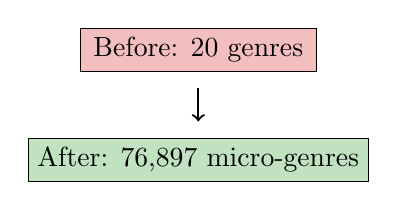
\begin{tikzpicture}[scale=0.7]
% Before
\node[draw,fill=mlred!30,minimum width=3cm] at (0,3) {Before: 20 genres};
% Arrow
\draw[->,thick] (0,2.3) -- (0,1.7);
% After
\node[draw,fill=mlgreen!30,minimum width=3cm] at (0,1) {After: 76,897 micro-genres};
\end{tikzpicture}
\end{center}

\textbf{Business Impact:}
\begin{itemize}
\item 75\% of views from recommendations
\item 18\% increase in engagement
\item 80\% catalog utilization (vs 40\%)
\item \$1B saved in content acquisition
\end{itemize}

\begin{tcolorbox}[colback=mlgreen!10, colframe=mlgreen]
\footnotesize
\textbf{Key Insight:} People don't want "action movies" - they want "Visually-striking nostalgic action dramas"
\end{tcolorbox}
\end{columns}

\bottomnote{Netflix's algorithm understands taste better than users understand themselves}
\end{frame}

% Slide 24: Spotify Micro-Moods
\begin{frame}[t]{Case Study: Spotify's 1,500 Micro-Moods}
\Large\textbf{Music Discovery Through Emotional Topics}
\normalsize

\vspace{0.5em}

\begin{columns}[T]
\column{0.48\textwidth}
\textbf{Traditional Categories:}
\begin{itemize}
\item Rock, Pop, Jazz, Classical
\item Happy, Sad, Energetic
\item Missing nuanced emotions
\end{itemize}

\vspace{0.5em}
\textbf{Topic Modeling on:}
\begin{itemize}
\item 4 billion playlists
\item Listening patterns by time
\item Skip rates and repeats
\item Playlist names and descriptions
\end{itemize}

\vspace{0.3em}
\textbf{Discovered Moods:}
\footnotesize
\begin{itemize}
\item "Monday motivation"
\item "Rainy day contemplation"
\item "Late night coding"
\item "Sunday morning coffee"
\item "Post-breakup empowerment"
\end{itemize}

\column{0.48\textwidth}
\textbf{The Innovation Map:}
\begin{center}
\includegraphics[width=0.9\textwidth]{charts/innovation_opportunity_map.pdf}
\end{center}

\textbf{Results:}
\begin{itemize}
\item 25\% increase in listening time
\item 40\% better playlist engagement
\item 31\% more diverse listening
\item 2.3B Discover Weekly streams
\end{itemize}

\begin{tcolorbox}[colback=mllavender4, colframe=mlpurple]
\footnotesize
\textbf{Innovation:} Created playlists for moods people couldn't name but instantly recognized
\end{tcolorbox}
\end{columns}

\bottomnote{Spotify creates 1 million personalized playlists every 24 hours using topic modeling}
\end{frame}

% Slide 25: 3M Innovation Mining
\begin{frame}[t]{Case Study: 3M's Patent Mining}
\Large\textbf{47 New Products from Hidden Connections}
\normalsize

\vspace{0.5em}

\begin{columns}[T]
\column{0.48\textwidth}
\textbf{The Challenge:}
\begin{itemize}
\item 100,000+ patents in portfolio
\item Siloed R\&D departments
\item Missing cross-applications
\item Duplicate research efforts
\end{itemize}

\vspace{0.5em}
\textbf{Topic Modeling Applied:}
\begin{itemize}
\item All patent descriptions
\item Research papers
\item Lab notebooks
\item Customer feedback
\end{itemize}

\vspace{0.3em}
\textbf{Unexpected Discoveries:}
\footnotesize
\begin{itemize}
\item Adhesive + Medical = Surgical tape
\item Abrasive + Dental = Tooth whitening
\item Reflective + Fashion = Safety clothing
\end{itemize}

\column{0.48\textwidth}
\textbf{Cross-Pollination Matrix:}
\begin{center}
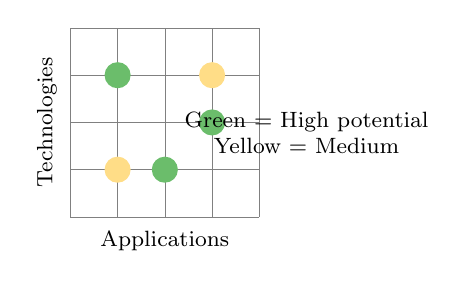
\begin{tikzpicture}[scale=0.6]
% Grid
\draw[step=1,gray,very thin] (0,0) grid (4,4);
% Labels
\node[rotate=90] at (-0.5,2) {\footnotesize Technologies};
\node at (2,-0.5) {\footnotesize Applications};
% Opportunities
\node[circle,fill=mlgreen!70] at (1,3) {};
\node[circle,fill=mlgreen!70] at (2,1) {};
\node[circle,fill=mlgreen!70] at (3,2) {};
\node[circle,fill=mlyellow!70] at (1,1) {};
\node[circle,fill=mlyellow!70] at (3,3) {};
\node at (5,2) {\footnotesize Green = High potential};
\node at (5,1.5) {\footnotesize Yellow = Medium};
\end{tikzpicture}
\end{center}

\textbf{Innovation Results:}
\begin{itemize}
\item 47 new product ideas identified
\item 12 launched within 18 months
\item \$120M revenue in year 1
\item 30\% reduction in R\&D redundancy
\end{itemize}
\end{columns}

\vspace{0.5em}
\begin{center}
\textcolor{mlpurple}{\textbf{Hidden connections in existing knowledge = breakthrough innovations}}
\end{center}

\bottomnote{3M now uses topic modeling on all research outputs to find innovation opportunities}
\end{frame}

% Slide 26: Customer Feedback Synthesis
\begin{frame}[t]{From Feedback Chaos to Product Roadmap}
\Large\textbf{Turning Complaints into Features}
\normalsize

\vspace{0.5em}

\begin{columns}[T]
\column{0.55\textwidth}
\begin{center}
\includegraphics[width=0.95\textwidth]{charts/topics_to_opportunities.pdf}
\end{center}

\column{0.43\textwidth}
\textbf{The Process:}
\begin{enumerate}
\footnotesize
\item Collect all feedback channels
\item Run topic modeling (LDA)
\item Identify pain point themes
\item Quantify impact
\item Prioritize solutions
\end{enumerate}

\vspace{0.5em}
\textbf{Example Topics → Features:}
\footnotesize
\begin{tabular}{ll}
\toprule
\textbf{Topic Found} & \textbf{Feature Built} \\
\midrule
"Confusing setup" & Onboarding wizard \\
"Battery anxiety" & Power-saving mode \\
"Lost features" & Search function \\
"Slow loading" & Cache system \\
\bottomrule
\end{tabular}

\vspace{0.5em}
\normalsize
\textbf{Impact:}
\begin{itemize}
\footnotesize
\item 40\% reduction in complaints
\item 28\% increase in retention
\item 50\% faster feature validation
\end{itemize}
\end{columns}

\bottomnote{Amazon analyzes 1 billion reviews yearly to drive product improvements}
\end{frame}

% Slide 27: IDEO Design Research
\begin{frame}[t]{Case Study: IDEO's Design Research Synthesis}
\Large\textbf{60\% Faster Insights, 3x More Patterns}
\normalsize

\vspace{0.5em}

\begin{columns}[T]
\column{0.48\textwidth}
\textbf{Traditional Research:}
\begin{itemize}
\item 100s of interviews
\item 1000s of sticky notes
\item Manual affinity mapping
\item 2-3 weeks synthesis
\item 5-10 insights found
\end{itemize}

\vspace{0.5em}
\textbf{With Topic Modeling:}
\begin{itemize}
\item Same interviews transcribed
\item LDA + NMF combination
\item Automatic theme discovery
\item 3 days to insights
\item 15-30 patterns found
\end{itemize}

\column{0.48\textwidth}
\textbf{Healthcare Project Example:}
\begin{center}
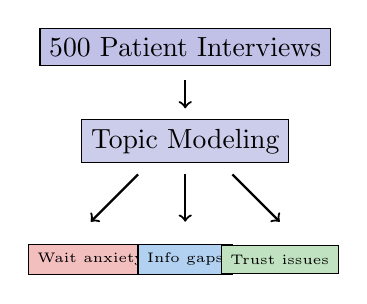
\begin{tikzpicture}[scale=0.6]
% Input
\node[draw,fill=mllavender2,minimum width=3cm] at (0,3) {500 Patient Interviews};
% Processing
\draw[->,thick] (0,2.3) -- (0,1.7);
\node[draw,fill=mllavender3,minimum width=2cm] at (0,1) {Topic Modeling};
% Output topics
\draw[->,thick] (-1,0.3) -- (-2,-0.7);
\draw[->,thick] (0,0.3) -- (0,-0.7);
\draw[->,thick] (1,0.3) -- (2,-0.7);
\node[draw,fill=mlred!30] at (-2,-1.5) {\tiny Wait anxiety};
\node[draw,fill=mlblue!30] at (0,-1.5) {\tiny Info gaps};
\node[draw,fill=mlgreen!30] at (2,-1.5) {\tiny Trust issues};
\end{tikzpicture}
\end{center}

\textbf{Insights Discovered:}
\footnotesize
\begin{itemize}
\item "Waiting room anxiety" → Redesigned space
\item "Information blackout" → Status system
\item "Provider trust" → Communication training
\end{itemize}

\normalsize
\textbf{Design Impact:}
\begin{itemize}
\item Patient satisfaction +34\%
\item Staff efficiency +22\%
\item Unexpected insights: 12
\end{itemize}
\end{columns}

\vspace{0.5em}
\begin{tcolorbox}[colback=mlgreen!10, colframe=mlgreen]
\centering
\textbf{IDEO's Secret:} Let algorithms find patterns, humans create meaning
\end{tcolorbox}

\bottomnote{Design thinking + machine learning = faster, deeper user understanding}
\end{frame}

% Slide 28: Building Innovation Pipeline
\begin{frame}[t]{Building Your Innovation Pipeline}
\Large\textbf{From Raw Data to Product Launch}
\normalsize

\vspace{0.5em}

\begin{columns}[T]
\column{0.48\textwidth}
\textbf{The 5-Step Process:}

\textbf{1. Data Collection}
\begin{itemize}
\footnotesize
\item Customer feedback
\item Market research
\item Competitor analysis
\item Patent databases
\end{itemize}

\textbf{2. Topic Discovery}
\begin{itemize}
\footnotesize
\item Run multiple algorithms
\item Validate with experts
\item Name and describe themes
\end{itemize}

\textbf{3. Opportunity Mapping}
\begin{itemize}
\footnotesize
\item Size each opportunity
\item Assess feasibility
\item Check market fit
\end{itemize}

\textbf{4. Prioritization}
\begin{itemize}
\footnotesize
\item Impact vs effort matrix
\item Resource requirements
\item Strategic alignment
\end{itemize}

\column{0.48\textwidth}
\textbf{The Innovation Funnel:}
\begin{center}
\includegraphics[width=0.9\textwidth]{charts/innovation_funnel_topics.pdf}
\end{center}

\textbf{Success Metrics:}
\begin{itemize}
\footnotesize
\item Ideas generated: 500+
\item Topics identified: 20-30
\item Opportunities validated: 5-10
\item Products launched: 1-3
\item Success rate: 60\% (vs 10\% traditional)
\end{itemize}
\end{columns}

\vspace{0.5em}
\begin{center}
\textcolor{mlpurple}{\textbf{Topic modeling turns information overload into innovation advantage}}
\end{center}

\bottomnote{Companies using topic modeling for innovation are 3x more likely to launch successful products}
\end{frame}
% Part 5: Practice & Case Study
\section{Practice: Real-world Application}

% Slide 1: Section Divider
\begin{frame}[plain]
\vfill
\centering
\begin{beamercolorbox}[sep=16pt,center]{title}
\usebeamerfont{title}\Large Part 5: Case Study \& Practice\\
\normalsize Amazon Review Intelligence System
\end{beamercolorbox}
\vfill
\end{frame}

% Slide 2: Case Study Introduction
\begin{frame}{Case Study: Amazon Review Intelligence}
\Large\textbf{Understanding 100 Million Customers}
\normalsize

\begin{columns}[T]
\begin{column}{0.55\textwidth}
\textbf{The Challenge:}
\begin{itemize}
\item 2+ million reviews daily
\item 35 languages
\item Multiple product categories
\item Fake review detection
\item Real-time insights needed
\end{itemize}

\vspace{0.5em}
\textbf{Business Goals:}
\begin{itemize}
\item Improve product quality
\item Identify trends early
\item Enhance customer satisfaction
\item Reduce return rates
\end{itemize}
\end{column}
\begin{column}{0.43\textwidth}
\includegraphics[width=0.85\textwidth]{charts/amazon_case_overview.pdf}
\end{column}
\end{columns}
\end{frame}

% Slide 3: Data Collection & Processing
\begin{frame}{Data Pipeline: Scale \& Speed}
\Large\textbf{Processing Millions of Reviews}
\normalsize

\begin{center}
\includegraphics[width=0.85\textwidth]{charts/amazon_data_pipeline.pdf}
\end{center}

\begin{columns}[T]
\begin{column}{0.32\textwidth}
\textbf{Collection}
\begin{itemize}
\small
\item Review text
\item Star ratings
\item Verified purchase
\item Product metadata
\item User history
\end{itemize}
\end{column}
\begin{column}{0.32\textwidth}
\textbf{Processing}
\begin{itemize}
\small
\item Language detection
\item Spam filtering
\item Text cleaning
\item Translation
\item Normalization
\end{itemize}
\end{column}
\begin{column}{0.32\textwidth}
\textbf{Analysis}
\begin{itemize}
\small
\item Sentiment scoring
\item Aspect extraction
\item Topic modeling
\item Trend detection
\item Anomaly flagging
\end{itemize}
\end{column}
\end{columns}
\end{frame}

% Slide 4: Sentiment Distribution Analysis
\begin{frame}{Sentiment Patterns: Beyond Star Ratings}
\Large\textbf{Text Reveals Hidden Insights}
\normalsize

\begin{columns}[T]
\begin{column}{0.55\textwidth}
\includegraphics[width=0.85\textwidth]{charts/sentiment_vs_stars.pdf}
\end{column}
\begin{column}{0.43\textwidth}
\textbf{Key Findings:}
\begin{itemize}
\item 23\% of 4-star reviews contain negative sentiment
\item 5-star reviews with ``but'' = future problems
\item 3-star most informative
\end{itemize}

\vspace{0.5em}
\textbf{Hidden Patterns:}
\begin{itemize}
\item Expectation mismatch
\item Feature complaints
\item Quality over time
\item Comparison mentions
\end{itemize}
\end{column}
\end{columns}

\begin{tcolorbox}[colback=mlorange!10,colframe=mlorange]
\centering
\small ``5 stars! Amazing product but the app could be better'' → Feature request identified
\end{tcolorbox}
\end{frame}

% Slide 5: Aspect-Based Analysis
\begin{frame}{Aspect-Based Sentiment: Granular Insights}
\Large\textbf{What Exactly Do They Love/Hate?}
\normalsize

\begin{center}
\includegraphics[width=0.85\textwidth]{charts/aspect_sentiment_matrix.pdf}
\end{center}

\textbf{Product: Echo Dot (Example)}
\begin{columns}[T]
\begin{column}{0.24\textwidth}
\textbf{Sound Quality}
\begin{itemize}
\small
\item Positive: 72\%
\item ``Clear voice''
\item ``Good bass''
\end{itemize}
\end{column}
\begin{column}{0.24\textwidth}
\textbf{Setup}
\begin{itemize}
\small
\item Negative: 45\%
\item ``Confusing''
\item ``WiFi issues''
\end{itemize}
\end{column}
\begin{column}{0.24\textwidth}
\textbf{Price}
\begin{itemize}
\small
\item Positive: 89\%
\item ``Great value''
\item ``Worth it''
\end{itemize}
\end{column}
\begin{column}{0.24\textwidth}
\textbf{Privacy}
\begin{itemize}
\small
\item Mixed: 50\%
\item ``Concerns''
\item ``Always listening''
\end{itemize}
\end{column}
\end{columns}
\end{frame}

% Slide 6: Key Insights & Patterns
\begin{frame}{Insights That Drive Product Changes}
\Large\textbf{From Analysis to Action}
\normalsize

\begin{columns}[T]
\begin{column}{0.55\textwidth}
\includegraphics[width=0.85\textwidth]{charts/insights_to_actions.pdf}
\end{column}
\begin{column}{0.43\textwidth}
\textbf{Top Discoveries:}
\begin{enumerate}
\item Setup wizard needed
\item Size expectations wrong
\item Packaging frustration
\item Feature discovery issue
\item Comparison shopping
\end{enumerate}

\vspace{0.5em}
\textbf{Actions Taken:}
\begin{itemize}
\item Redesigned onboarding
\item Added size reference
\item Simplified packaging
\item Created tutorials
\item Comparison tool
\end{itemize}
\end{column}
\end{columns}
\end{frame}

% Slide 7: Impact & Results
\begin{frame}{Results: Measurable Improvement}
\Large\textbf{ROI of Sentiment Analysis}
\normalsize

\begin{center}
\includegraphics[width=0.85\textwidth]{charts/improvement_metrics.pdf}
\end{center}

\begin{columns}[T]
\begin{column}{0.48\textwidth}
\textbf{Customer Metrics:}
\begin{itemize}
\item Return rate: -18\%
\item Support tickets: -35\%
\item Satisfaction: +12\%
\item Repeat purchase: +22\%
\end{itemize}
\end{column}
\begin{column}{0.48\textwidth}
\textbf{Business Impact:}
\begin{itemize}
\item \$50M saved in returns
\item 2x faster issue detection
\item 40\% better forecasting
\item 25\% higher LTV
\end{itemize}
\end{column}
\end{columns}
\end{frame}

% Slide 8: Practice Exercise
\begin{frame}{Practice Exercise: Twitter Sentiment Analysis}
\Large\textbf{Your Turn: Analyze Brand Perception}
\normalsize

\begin{columns}[T]
\begin{column}{0.48\textwidth}
\textbf{Dataset:}
\begin{itemize}
\item 5,000 tweets about a product
\item Last 30 days
\item Multiple languages
\item Includes replies/mentions
\end{itemize}

\vspace{0.5em}
\textbf{Tasks:}
\begin{enumerate}
\item Clean and preprocess
\item Sentiment classification
\item Emotion detection
\item Topic extraction
\item Temporal analysis
\item Create insights report
\end{enumerate}
\end{column}
\begin{column}{0.48\textwidth}
\textbf{Deliverables:}
\begin{itemize}
\item Jupyter notebook
\item Sentiment dashboard
\item Top 10 pain points
\item Emotion journey map
\item Recommendations
\end{itemize}

\vspace{0.5em}
\textbf{Bonus Challenges:}
\begin{itemize}
\item Detect sarcasm
\item Find influencers
\item Predict virality
\item Compare competitors
\end{itemize}
\end{column}
\end{columns}

\vspace{0.5em}
\begin{tcolorbox}[colback=mlgreen!10,colframe=mlgreen]
\centering
\textbf{Time:} 2 hours | \textbf{Tools:} Python, BERT, Plotly | \textbf{Goal:} Actionable insights
\end{tcolorbox}
\end{frame}

% Slide 9: Key Takeaways
\begin{frame}{Week 3 Key Takeaways}
\Large\textbf{What You've Learned}
\normalsize

\begin{columns}[T]
\begin{column}{0.48\textwidth}
\textbf{Technical Skills:}
\begin{itemize}
\item Text preprocessing pipelines
\item BERT implementation
\item Sentiment classification
\item Emotion detection
\item Production deployment
\end{itemize}

\vspace{0.5em}
\textbf{Tools Mastered:}
\begin{itemize}
\item Hugging Face Transformers
\item spaCy/NLTK
\item FastAPI
\item Pandas/NumPy
\end{itemize}
\end{column}
\begin{column}{0.48\textwidth}
\textbf{Design Applications:}
\begin{itemize}
\item Voice of Customer analysis
\item Emotional journey mapping
\item Pain point prioritization
\item Feature discovery
\item Impact measurement
\end{itemize}

\vspace{0.5em}
\textbf{Business Value:}
\begin{itemize}
\item Scalable insights
\item Real-time monitoring
\item Data-driven decisions
\item Customer empathy
\end{itemize}
\end{column}
\end{columns}

\vspace{0.5em}
\begin{tcolorbox}[colback=mlblue!10,colframe=mlblue]
\centering
\Large\textbf{Next Week:} Classification for Problem Definition
\end{tcolorbox}
\end{frame}

% Closing slide
\begin{frame}[plain]
\vspace{2cm}
\begin{center}
{\Huge \textcolor{mlpurple}{\textbf{Topic Modeling Mastered}}}\\[1cm]
{\Large You Can Now:}\\[0.5cm]
{\normalsize
\begin{itemize}
\item Find hidden themes in massive text collections
\item Choose the right algorithm for your data
\item Transform unstructured feedback into structured insights
\item Discover innovation opportunities others miss
\end{itemize}
}
\vspace{1cm}
{\large \textcolor{mlpurple}{\textbf{Next Week: Generative AI for Rapid Prototyping}}}
\end{center}
\end{frame}

\end{document}